%\documentclass{article}


\documentclass[12pt]{article}
\usepackage{graphicx} % This lets you include figures
\usepackage{hyperref} % This lets you make links to web locations

\usepackage[brazil]{babel}
\usepackage[utf8]{inputenc}

\graphicspath{ {./images/} }

\usepackage[rightcaption]{sidecap}
\usepackage{subcaption}
\usepackage{wrapfig}

\usepackage{float}

\usepackage{imakeidx}
\usepackage{listings}
\usepackage[bottom]{footmisc}
\usepackage{todonotes}
\usepackage{blindtext}

\makeindex

\title{Sistema de busca de artigos e monografias}
\author{UnB-FGA}
\date{\today}

\begin{document}
\maketitle{}

\tableofcontents

\clearpage
\newpage

\section{Introdução}

\subsection{Oracle VM VirtualBox}\label{vbox}

\begin{wrapfigure}{r}{0.2\textwidth} %this figure will be at the right
    \centering
    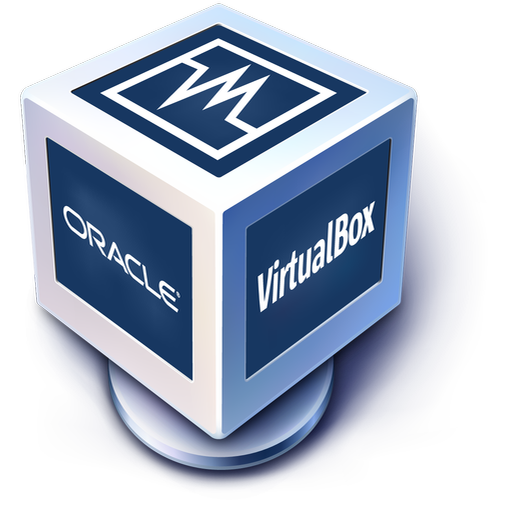
\includegraphics[width=0.2\textwidth]{../images/vbox.png}
\end{wrapfigure}

VirtualBox é um software de virtualização que pode ser instalado em diversos sistemas hospedeiros e tem como objetivo gerenciar máquinas virtuais.

Para este manual, a versão do VirtualBox que está sendo executado é a 6.0.8 em um hospedeiro Windows, e foi o software escolhido para executar a imagem do ambiente Linux Alpine onde é executado o sistema de buscas.

Após a instalação do software\footnotetext{\url{https://www.virtualbox.org/wiki/Downloads}} e dada uma imagem \lstinline{.ova}, para replicar o ambiente no VirtualBox, é necessário:
\begin{enumerate}
    \item Escolher a opção do menu \textit{Import Appliance}.
     \begin{figure}[h]
        \centering
        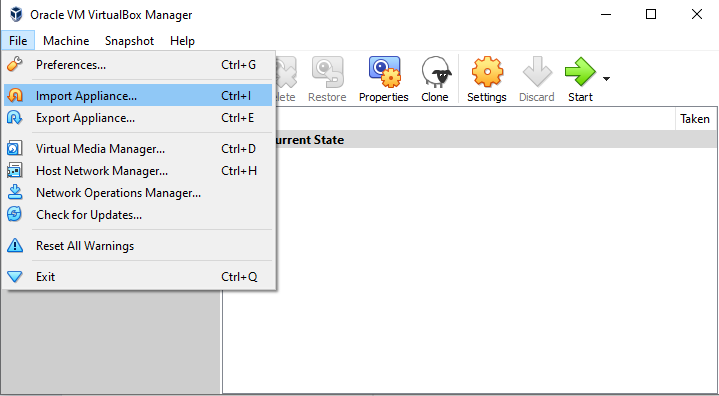
\includegraphics[width=0.5\textwidth]{images/vbox1.png}
    \end{figure}
    \item Escrever o caminho da imagem do Alpine \lstinline{.ova}.
    \item Selecionar a opção \textit{Import} para uma importação básica do sistema. Após esse processo, espere o processo de importação terminar.
\end{enumerate}

Se a imagem foi instalada corretamente, clique em \textit{Start} no menu principal do VirtualBox e aguardea tela de boas vindas ilustrada na Figura \ref{fig1}.
\begin{figure}[h]
    \centering
    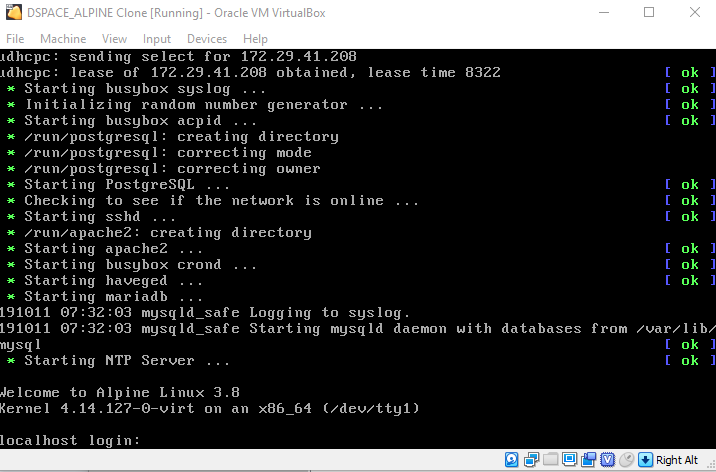
\includegraphics[width=0.5\textwidth]{images/vbox2.png}
    \caption{Tela de Boas-Vindas.}
    \label{fig1}
\end{figure}

Considerando que nenhuma outra configuração no VirtualBox foi feita além das explicadas neste manual, utilize a tecla \textit{AltGr} para alternar o foco entre o sistema hospedeiro e o sistema cliente. 

\subsection{Alpine Linux}\label{alpine}

 \begin{wrapfigure}{r}{0.2\textwidth} %this figure will be at the right
     \centering
     
\includegraphics[width=0.2\textwidth]{../images/alpine.png}
     \label{fig2}
 \end{wrapfigure}

Alpine é uma distribuição Linux para uso não-comerciais, com o foco em eficiência e simplicidade, possuindo apenas recursos básicos e necessários para o ambiente Linux.

A versão utilizada neste sistema é a 3.8, sendo uma imagem de extensão \lstinline{.ova}, que pode ser simulada no programa VirtualBox, explicado na Seção \ref{vbox}. Assim que o sistema é inicializado, é exigido um login e uma senha para utilizar o ambiente. 

\begin{lstlisting}[language=bash, label=lst1, caption=Login e senha de acesso]
    localhost login: dspace
    Password: dspace
\end{lstlisting}

Os principais programas que inicializam juntamente com o Alpine são:

\begin{itemize}
    \item PostgreeSQL, seção \ref{postgree}
    \item Apache, seção \ref{apache}
    \item MariaDB, seção \ref{mariadb}
\end{itemize}

Para utilizar os recursos do Alpine na máquina hospedeira, recomenda-se o programa Putty, explicado na Seção \ref{conexao}.

Para transferir arquivos entre a máquina hospedeira e o Alpine, recomenda-se o programa Filezilla, explicado na Seção \ref{transfer}.

\subsubsection{Gerenciamento de pacotes}

O Alpine utiliza o sistema de gerenciamento de pacotes \lstinline{apk}, que pode ser lido em mais detalhes em \url{https://wiki.alpinelinux.org/wiki/Alpine_Linux_package_management}.

A lista dos repositórios de pacotes disponíveis do Alpine podem ser editados utilizando o editor \textit{vim} com o comando:

\begin{lstlisting}[language=bash]
    vim /etc/apk/repositories
\end{lstlisting}

Atualmente, a versão dos repositórios escolhidos para baixar os pacotes é a \textbf{3.3}, disponíveis em \url{http://mirror.math.princeton.edu/pub/alpinelinux/}, que até o momento possuía o pacote \textbf{php-apache} e o pacote \textbf{php-mysql}, os quais foram essenciais para a instalação do sistema Tematres, explicado na Seção \ref{tematres}.

\subsubsection{Conexão entre máquina hospedeira e a imagem}\label{conexao}

\begin{wrapfigure}{r}{0.2\textwidth} %this figure will be at the right
    \centering
    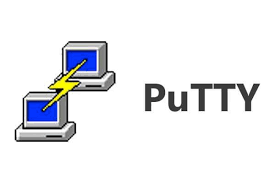
\includegraphics[width=0.2\textwidth]{../images/putty1.png}
\end{wrapfigure}

Putty é um software de emulação de terminal que suporta conexões SSH e telnet. Desta forma, fica mais simples manipular o cliente, no caso deste manual, o Alpine, sem necessariamente utilizar a máquina virtual, a qual está rodando no VirtualBox.

Para utilizar o Putty juntamente com a imagem do Alpine disponibilizada, utilize o comando \lstinline{ifconfig} para descobrir o endereço \textit{inet} e fazer a conexão entre o Putty e o terminal do alpine.

 \begin{figure}[h]
 
     \begin{subfigure}{0.6\textwidth}
     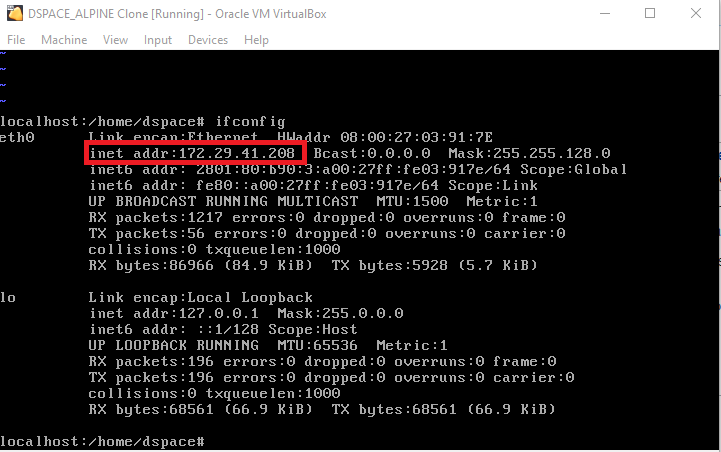
\includegraphics[width=0.9\linewidth]{../images/putty2.png} 
     \caption{ifconfig.}
     \end{subfigure}
     \begin{subfigure}{0.4\textwidth}
     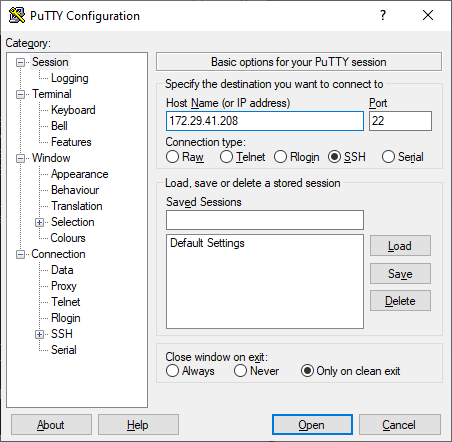
\includegraphics[width=0.9\linewidth]{../images/putty3.png}
     \caption{Configuração do putty.}
     \end{subfigure}
 
 \caption{Utilizando Putty.}
 \end{figure}

 No Putty, edite o campo \textit{Host Name (or IP adress)} com o endereço \textit{inet} fornecido, confira se a porta selecionada é a \textit{22} e se o tipo de conexão é \textit{SSH}. Após isso, clique em \textbf{Open}.

 Irá aparecer um aviso sobre conexão não-segura, o qual pode ser ignorado. O login e a senha serão os mesmos informados na Listagem \ref{lst1}.

 \begin{figure}[h]
    \centering
    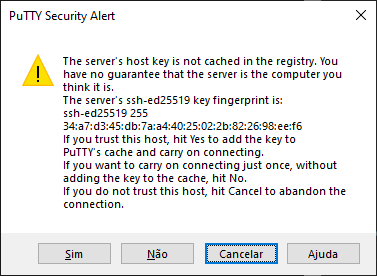
\includegraphics[width=0.5\textwidth]{images/putty4.png}
    \caption{Aviso de conexão não-segura. Clique em \textit{sim} para ignorar.}
    \label{fig1}
\end{figure}

Após isso, você poderá utilizar o terminal do Alpine na máquina hospedeira.

\subsubsection{Transferência de arquivos}\label{transfer}

\subsection{PostgreeSQL}\label{postgree}

\todo{O que é} \blindtext

\todo{onde é usado} \blindtext

\todo{como conectar} \blindtext

\subsection{Apache}\label{apache}

\todo{O que é} \blindtext

\todo{onde é usado} \blindtext

\todo{como conectar} \blindtext

\subsection{MariaDB}\label{mariadb}

\todo{O que é} \blindtext

\todo{onde é usado} \blindtext

\todo{como conectar} \blindtext

% \begin{wrapfigure}{r}{0.5\textwidth}
%     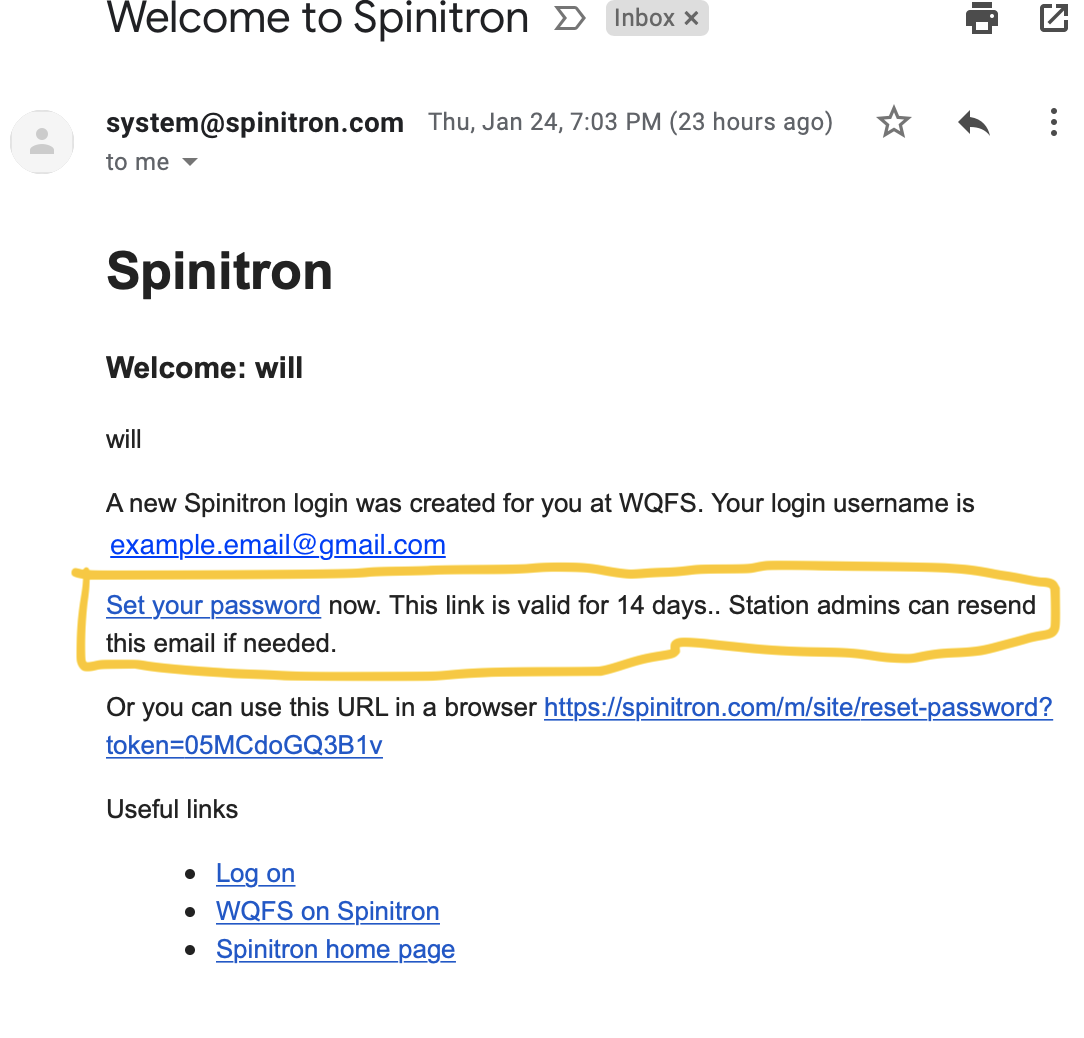
\includegraphics[width=0.5\textwidth]{images/email.png}
%     \caption{Note the link expires after 14 days.}
%     \label{fig2}
% \end{wrapfigure}

% Go to your email and click or copy the link provided by Spinitron. 
% This email should look like Figure~\ref{fig2}

% Remember your email will be your login username.

% Create your password on the page that the link takes you to.

% {\it Please do not forget your password.}

% \clearpage
% \newpage

% \subsection{Logging In}

% %\begin{wrapfigure}{r}{0.45\textwidth}
% %    \includegraphics[width=0.45\textwidth]{images/login_after_password.png}
% %    \caption{The log-in screen.}
% %    \label{fig3}
% %\end{wrapfigure}

%  Next, once you have created your new password Spinitron will take you a page that should look like Figure~\ref{fig3a}. 

% It should say ``New password saved.''

% This is the log-in screen. Enter your email address and password to log in.

% NOTE: sometimes Spinitron will take you to the old version of the website. If that happens, simply click the link that says ``Login for Spinitron v2 is here'' as seen in Figure~\ref{fig3b}

% \begin{figure}[h]
 
%     \begin{subfigure}{0.6\textwidth}
%     \includegraphics[width=0.9\linewidth]{images/login_after_password.png} 
%     \caption{The log-in screen.}
%     \label{fig3a}
%     \end{subfigure}
%     \begin{subfigure}{0.4\textwidth}
%     \includegraphics[width=0.9\linewidth]{images/old_version.png}
%     \caption{The old version of Spinitron.}
%     \label{fig3b}
%     \end{subfigure}
 
% \caption{Login screens.}
% \label{fig:image2}
% \end{figure}

% %\begin{figure}[h]
% %\includegraphics[width=0.40\textwidth]{images/old_version.png}
% %\caption{The old version of Spinitron.}
% %\label{fig4}
% %\end{figure}



% \subsection{Home-Screen and Setup}

% \begin{wrapfigure}{r}{0.45\textwidth}
%     \includegraphics[width=0.45\textwidth]{images/phone_banner.png}
%     \caption{The set phone number banner takes you to the User account page.}
%     \label{fig4}
% \end{wrapfigure}

% Now you are on the Spinitron DJ Home screen. 
% It should look like Figure~\ref{fig4}

% Setup your User account by selecting ``User account'' under the drop-down box under your DJ name or click the ``Please set your phone number.'' banner.

% Make sure you put the correct phone number, this is the number that managers will use to contact you in the future.

% \clearpage
% \newpage

% \subsection{DJ profile}

% (OPTIONAL) Setup your DJ profile. This is accessed using the drop-down box under your DJ name in the top right corner of the page. 
% You can put as much or little information as you like.

% NOTE: Spinitron uses random photos for anything you do not put in a picture for, you are welcome to leave them as they are, delete them, or replace them.

% \begin{figure}[h]
%     \centering
%     \includegraphics[width=0.5\textwidth]{images/Dropdown.png}
%     \caption{The drop-down}
%     \label{fig5}
% \end{figure}

% \begin{figure}[h]
 
%     \begin{subfigure}{0.5\textwidth}
%     \includegraphics[width=1.0\linewidth, height=5cm]{images/DJ_profile1.png} 
%     \label{fig:DJp1}
%     \end{subfigure}
%     \begin{subfigure}{0.5\textwidth}
%     \includegraphics[width=1.0\linewidth, height=5cm]{images/DJ_profile2.png}
%     \label{fig:DJp2}
%     \end{subfigure}
 
% \caption{The DJ profile page}
% \label{fig6}
% \end{figure}
 \clearpage
 \newpage
\section{Softwares utilizados}
\subsection{Dspace}\label{dspace}

\todo{O que é} \blindtext

\todo{onde é usado} \blindtext

\todo{como instalar} \blindtext

\subsection{Tematres}\label{tematres}

\begin{wrapfigure}{r}{0.2\textwidth} %this figure will be at the right
    \centering
    
\includegraphics[width=0.2\textwidth]{../images/tematres.jpg}
\end{wrapfigure}

Tematres é uma ferramenta para controlar vocábulos controlados e taxonomias. Suporta análise e categorização de termos de busca através de metadados, fornecendo uma interface web para realizar este controle.

Como é um sistema em PHP, ele atualmente está instalado no diretório \textit{localhost}, que pode ser acessado através do caminho exibido na Listagem \ref{lst:tematres.caminho}.
\begin{lstlisting}[language=bash, label=lst:tematres.caminho, caption=Instalação do Tematres.]
    /var/www/localhost/htdocs/tematres
\end{lstlisting}

Para acessar a página de instalação do tematres, acesse a URL disponível na Listagem \ref{lst:tematres.url}
\begin{lstlisting}[language=bash, label=lst:tematres.url, caption=Instalação do Tematres.]
    <ENDERECO INET>/tematres
\end{lstlisting}

 \clearpage
 \newpage
 \section{Sistema de busca}
\subsection{Sistema de busca de monografias}\label{dspace}

\todo{Motivação} \blindtext

\todo{como usar} \blindtext





% \clearpage
% \newpage

% \section{Setting up your Show and Playlists:}


% \subsection{Creating a Show Slot in the Schedule}

% \begin{wrapfigure}{r}{0.4\textwidth}
%     \includegraphics[width=0.4\textwidth]{images/Schedule.png}
%     \caption{The Schedule page}
%     \label{fig7}
% \end{wrapfigure}

% Click on the schedule tab in the menu bar at the top of the web-page.
% Find your date and time on the calendar and click on that slot. (For this example I will be creating a show on Saturday mornings at 2am.)

% Then click ``new show''.

% \hrulefill

% This step is important as it creates a reoccurring show that your playlist is attached to. This helps listeners and managers find your other playlists, as well as, helping keep the station organized.

% \hrulefill

% \vspace{1cm}

% \subsection{Creating a New Show}

% You should now see a blank form that looks like this:

% \begin{figure}[h]
 
%     \begin{subfigure}{0.5\textwidth}
%     \includegraphics[width=0.9\linewidth, height=5cm]{images/New_show1.png} 
%     \label{fig:NS1}
%     \end{subfigure}
%     \begin{subfigure}{0.5\textwidth}
%     \includegraphics[width=0.9\linewidth, height=5cm]{images/New_show2.png}
%     \label{fig:NS2}
%     \end{subfigure}
 
% \caption{The New Show Form.}
% \label{fig8}
% \end{figure}

% \clearpage

% \begin{wrapfigure}{r}{0.5\textwidth}
%     \includegraphics[width=0.5\textwidth]{images/New_show3.png}
%     \caption{The duration has been changed to 120 and a Co-DJ has been added.}
%     \label{fig9}
% \end{wrapfigure}


% Fill out the show information and REMEMBER to set your show duration to 120 minutes as we have 2 hour slots.

% The Description box is a great place to talk about what kind of music you like to play on your show or if you have a specialty show etc. 

% If you have a Co-DJ then you can add them under DJs as has been done in this example. If you do not have a co-DJ, then you can leave the DJs box alone. It should have auto-filled your name along with your DJ name in parenthesis.

% Do not click on either of the check-boxes, they should be left unchecked as seen in Figure~\ref{fig9}.

% Once you are happy with your show's information and have changed the Duration to 120, go to the bottom of the page and click on the gear icon as shown in Figure~\ref{fig10} 
% to check that: your show repeats weekly, is at the right time, and is on the correct day. 

% Then hit ``Save''

% You can edit this later if you forgot something or have done something wrong.
% (Covered in section~\ref{show_page})

% \begin{figure}[h]
%     \centering
%     \includegraphics[width=0.5\textwidth]{images/New_show_saving_options.png}
%     \caption{The gear icon and the save button on the New Show page.}
%     \label{fig10}
% \end{figure}

% \subsection{The Show page:} \label{show_page}

% \begin{wrapfigure}{r}{0.5\textwidth}
%     \includegraphics[width=0.5\textwidth]{images/New_show_page.png}
%     \caption{The Show page.}
%     \label{fig11}
% \end{wrapfigure}

% You should now see a page that looks similar to this: 

% \hrulefill

% NOTE:
% You can see what your show page looks like to listeners by clicking on the Public page button.

% If anything appears to be incorrect, you can edit or update it with the edit show button.

% \hrulefill

% Click on the green ``Create Playlist'' button at the top of the page.

% \subsection{Creating a Playlist:}
% Now you will see a page that looks very similar to the create show page as seen in Figure~\ref{fig12}.
% {\it It is required from NOW ON that the date should come at the end of your playlist's name. }

% This will help you as well as the managers differentiate between the numerous shows that will accumulate under the same or very similar names.

% \hrulefill

% PLEASE end the name of your playlists with the DATE they are aired.

% For example:

% ``The Sunday Afternoon EDM show 1/27/19''

% or ``Sabrina's Hip-hop and House Episode\#3 Jan, 8''

% or ``Will's show 4.13.2019''

% \hrulefill

% Until further notice all other organization such as Episode Name and Description are optional.

% \begin{figure}[H]
%     \centering
%     \includegraphics[width=0.5\textwidth]{images/New_Playlist_naming_date.png}
%     \caption{Please end your playlist's name with the date it is aired}
%     \label{fig12}
% \end{figure}

% \subsection{Creating Additional Playlists:}

% \begin{wrapfigure}{r}{0.5\textwidth}
%     \includegraphics[width=0.5\textwidth]{images/Second_Playlist.png}
%     \caption{Click the link that is the name of your show.}
%     \label{fig13}
% \end{wrapfigure}

% To create your second, third, etc. playlists for your show, go to the drop-down under ``Playlist'' and your show's name should appear under ``New playlist for...'' as seen in Figure~\ref{fig13}

% Click on your show's name there. This will create another playlist for that show.

% Select the correct date and time, and make sure to add the date to the end of the playlist name.

% (Optional) Fill out any other information.

% \clearpage
% \newpage

% \section{Using Spinitron:}

% \subsection{Playlist Entry Form.}

% \begin{wrapfigure}{r}{0.5\textwidth}
%     \includegraphics[width=0.5\textwidth]{images/Playlist_entry_form.png}
%     \caption{The playlist entry form.}
%     \label{fig14}
% \end{wrapfigure}


% After Creating a playlist you should now see a page that looks like Figure~\ref{fig14}

% This is how you will enter spins into Spinitron. 

% The only REQUIRED fields are: 
% \\
% Song, Artist, and Rotation (if the song is in rotation)
% \\
% NOTE: Do not mark a song that is not rotation as rotation!

% \vspace{1cm}

% \begin{figure}[h]
%     \centering
%     \includegraphics[width=1\textwidth]{images/Playlist_entry_form_marked1.png}
%     \caption{Required Fields.}
%     \label{fig15}
% \end{figure}

% \clearpage

% \subsection{Using the Playlist Entry Form:}

% Simply start typing in the name of the artist in the ``Artist'' box,
% if it appears in the auto-fill you can (and should) click on it.

% Next type in the song name in the ``Song'' box,
% if it appears in the auto-fill you can (and should) click on it.

% Then if and only if, the song is in rotation, click on the ``Rotation:'' drop-down box and select the correct rotation (A, B, C, or NC)

% You can fill out as much or little other information as you wish. Also there is a text-box labeled ``Song note'' in which you can add any notes or other information on the song that you might wish to include.

% After you have done these things, click on either the ``Submit'' or ``Cue'' button on the bottom left as seen in Figure~\ref{fig15}.

% \subsection{The ``Cue'' and ``Submit'' Functions.}

% It is recommended that you use the ``Cue'' function when adding spins. 

% The ``Cue'' function works by adding your song to the list but not time-stamping it. This allows you to be several songs ahead as you can cue up as many spins as you want ahead of time. {\it The order spins are cued does not matter!} After cueing a spin(s) you can submit a spin, cue more spins, time-stamp a cued spin, or cue non-music spins. 

% To time-stamp and ``Activate'' a Cued spin, look down to where the spin appears after having been cued, it should appear in yellow with a ``Now'' button next to the empty time-stamp slot. Clicking on the ``Now'' button time-stamps the cued spin to the current time, it will then change color from yellow to white/gray and it will also be visible on the public version of your playlist page. 


% The ``Submit'' function works by submitting a song and time-stamping it to whatever time is in the start box on the left side of the screen this is set as a default to the current time. (the time can be adjusted using the gear icon in the top right corner, Ex: being set to the time-stamp of last spin + last spin duration which is helpful for adding old playlists to the Spinitron website.) 

% Time-stamps are how Spinitron organizes spins, and it will not display spins that do not have a time-stamp so you need to try to: 
% \\
% 1. Have all your spins time-stamped 
% \\
% 2. Attempt to have the time-stamps to be as accurate as possible (using the cue function makes this much easier)


% NOTE: If you use the auto-fill function it will add album artwork and other information that makes your public page prettier and more interesting for everyone.

% %Sometimes Spinitron will present a window that asks if you meant one version of a song or another, select the correct or closest to correct version. If you cannot tell the difference or do not know which one is correct, then just pick one or ignore.

% \subsection{Entering ``non-music items:''}

% \begin{figure}[h]
%     \centering
%     \includegraphics[width=1\textwidth]{images/Add_non-music.png}
%     \caption{This is how you add non-music items.}
%     \label{fig16}
% \end{figure}


% Logging non-music entries, (such as PSAs, the Station ID, and Voice Breaks) is done by clicking the ``Add non-music item'' drop-down in the top right corner of the web-page and selecting the appropriate item as seen in Figure~\ref{fig16}.


% If you have selected the Station ID non-music item then, this will change the Playlist Entry Form screen to look like Figure~\ref{fig17}. 
% The other items look similar but have different features such as editable ``Description'' box for PSAs and Voice Breaks that allows you to describe what PSA you played, or to describe your Voice Break. 

% Voice Breaks also have an editable ``Title'' box so you can label your voice breaks.

% There are also two check boxes at the bottom of the Station ID form. The ``Public'' and ``Signature'' boxes.

% \begin{wrapfigure}{r}{0.5\textwidth}
%     \includegraphics[width=0.5\textwidth]{images/StationID.png}
%     \caption{The Station ID non-music item form.}
%     \label{fig17}
% \end{wrapfigure}

% If the ''Public'' box is checked, people looking at your playlist will be able to see this item. If it is not checked, they will not.

% If the ``Signature'' box is your signature that you have played/spoken this item, some items will not be able to be submitted if you do not check this box.

% \hrulefill

% If you check the ``Signature'' box without having played said item and then submit that item, you are being dishonest. 
% \\
% THIS IS A STRIKE OFFENSE.

% \hrulefill

% % NOTE:







% \section{Advanced features:}

% \subsection{Coming Soon:}

% Most of these features can be found on the Spinitron website under ``About'' on the top left and then ``Getting started - DJs'' on the left side. 
% \href{https://spinitron.com/about/help/get-started-dj.html}{{\it OOOOOR at this link right here!}}

% \subsection{Importing Playlists:}

% This works very well with Itunes.
% Link to YouTube video containing this is: 
% \href{https://www.youtube.com/watch?v=aN8mCR1NiHc}{{\it Import a Playlist}}

% \subsection{Playlist worksheet features: This EXPLAINS THE CUE FUNCTION!}

% Link to YouTube video containing this is:
% \href{https://www.youtube.com/watch?v=xj7dVbhUXFM}{{\it Playlist worksheet features}}

% \subsection{Covering for another DJ:}

% \newpage

% \section{Links:}

% \subsection{Login:}

% \url{https://spinitron.com/m/site/login}

% \subsection{Help getting started:}

% \url{https://spinitron.com/about/help/get-started-dj.html}

% \subsection{The Spinitron YouTube channel:}

% \url{https://www.youtube.com/channel/UCoqehWXhiILwXznsnn8CblA}


%\href{http://class.guilford.edu/physics/dasmith}{this way}

%\footnote{You can put the link in a footnote like this.}

% Anything to the right of a percent sign will be ignored by LaTeX.
% You can use this to put notes to yourself.  If you want to actually
% get a percent sign in your PDF file, use \%.  This holds for many 
% symbols, like \$ and \&.  Without the backslash, LaTeX will think
% you are trying to give it a command, and it will get confused.
% Note that this paragraph does not show up in the PDF.

\newpage

\listoffigures

\end{document}
